\setchapterimage[6cm]{chapter/aircraft/aircraft_title_photo2.jpg}
\setchapterpreamble[u]{\margintoc}
\chapter{Aircraft from small to large\protect\footnotemark}
\labch{aircraft-chapter_en}

\footnotetext{\href{https://en.wikipedia.org/wiki/NASA_X-43}{NASA X-43} it is the fastest aircraft in the history of aviation.
Author: \href{https://commons.wikimedia.org/wiki/File:X43a2_nasa_scramjet.jpg}{NASA, WikiCommons / 2008 / public domain}. }

The chapter is devoted to the study of various properties of aircraft
based on Wikidata.
In the course of research using SPARQL queries calculated on objects of the type ``Aircraft",
received information about all aircraft and their number,
also a diagram showing the ratio of the total number of aircraft manufacturers by country was obtained.
The chapter concludes with an estimate of the completeness of the data presented in Wikipedia and Wikidata. According to her, Wikidata contains only
300 records of aircraft manufacturers out of \num{1700}.

%%%%%%%%%%%%%%%%%%%%%%%%%%%%%%%%%%%%%%%%%%%%%%%%%%%%%%%

\section{Instances of the object ``Aircraft"}

Let's build a list of all instances of the object ``Aircraft" \href{https://www.wikidata.org/wiki/Q11436}{Q11436}.

\begin{lstlisting}[ language=SPARQL, breaklines=true, 
                    caption={List of aircrafts\\\hspace{\textwidth}
                        The result contains \num{1564} aircrafts in 2017, 
                        \num{3324} aircrafts in 2020.\\\hspace{\textwidth}
                        SPARQL query: \href{https://w.wiki/nZU}{w.wiki/nZU}
                        },
                    label=lst:aircraft_listing_1,
                    texcl 
                    ]
#List of `instances of` "aircraft"
#Q11436 - object aircraft 
#P31 - properties instance of
SELECT ?item ?itemLabel
WHERE
{
    ?item wdt:P31 wd:Q11436. # instances of aircraft
    SERVICE wikibase:label {bd:serviceParam wikibase:language "en"}
}
\end{lstlisting}

The most complete and well-developed aircraft on Wikidata for 2017 are: \href{https://www.wikidata.org/wiki/Q271446}{Mikoyan-Gurevich MiG-3}, 
\href{https://www.wikidata.org/wiki/Q1349098}{Yakovlev Yak-36}, \href{https://www.wikidata.org/wiki/Q429839}{Mitsubishi A5M}. 
For 2020, the most complete and well-developed aircraft on Wikidata are: \href{https://www.wikidata.org/wiki/Q770863}{Sopwith Triplane} (18 properties), 
\href{https://www.wikidata.org/wiki/Q1658673}{IL-103} (14 properties), \href{https://www.wikidata.org/wiki/Q665071}{Martin 2-0-2} (14 properties).
Almost empty and uninformative aircraft for 2017 turned out to be: \href{https://www.wikidata.org/wiki/Q464247}{Mikoyan-Gurevich MiG-1}, 
\href{https://www.wikidata.org/wiki/Q2296502}{Sukhoi Su-6}, \href{https://www.wikidata.org/wiki/Q1658673}{Il-103}.
For 2020, uninformative aircraft are: \href{https://www.wikidata.org/wiki/Q820603}{Beriev Be-1} (3 properties), \href{https://www.wikidata.org/wiki/Q117984}{Lituanica} (4 properties), 
\href{https://www.wikidata.org/wiki/Q572762}{Lavochkin La-168} (3 properties).

%%%%%%%%%%%%%%%%%%%%%%%%%%%%%%%%%%%%%%%%%%%%%%%%%%%%%%%

\section{Aircraft manufacturers}

Let's make a list of aircraft manufacturers.

\index{SPARQL!COUNT / Aircraft manufacturers}
\begin{lstlisting}[ language=SPARQL, breaklines=true, 
                    caption={Aircraft manufacturers\\\hspace{\textwidth}
                        The result contains \num{300} manufacturers in 2017, 
                        \num{597} manufacturers in 2020.\\\hspace{\textwidth}
                        SPARQL query: \href{https://w.wiki/nZZ}{w.wiki/nZZ}
                        },
                    label=lst:aircraft_listing_2,
                    texcl 
                    ]
# Count aircraft having property manufacture, group by manufacture
SELECT ?manufactureLabel (COUNT(?item) AS ?count) 
WHERE {
  ?item wdt:P31 wd:Q11436.     # instance of aircraft
  ?item wdt:P176 ?manufacture. # show manufacture
  SERVICE wikibase:label {bd:serviceParam wikibase:language "en".}
}
GROUP BY ?manufacture ?manufactureLabel 
\end{lstlisting}

The result of the query~\ref{lst:aircraft_listing_2} is a list of all aircraft manufacturers.

%%%%%%%%%%%%%%%%%%%%%%%%%%%%%%%%%%%%%%%%%%%%%%%%%%%%%%%

\label{question:aircraft_manufacturers_en}
\marginnote{
Which Russian aircraft manufacturers have websites?
\begin{itemize}
\item MiG
\item Saratov Aviation Plant
\item Tupolev
\item Sukhoi
\end{itemize}
The answer is on page~\pageref{answer:aircraft_manufacturers_en}.
}


\section{Number of aircraft produced}

\index{Aircraft!Aviation industry / definition}
The aviation industry is one of the largest mechanical engineering industries in the world. Its tasks include both the development 
and production of various aerial vehicles. In order to assess which aircraft models are the most widespread, we will build a diagram 
of the produced aircraft of various models.

\begin{lstlisting}[ language=SPARQL, breaklines=true, 
                    caption={List of aircraft and their number produced\\\hspace{\textwidth}
                        The result contains \num{177} records in 2020. 
                        SPARQL query: \href{https://w.wiki/nZF}{w.wiki/nZF}
                        },
                    label=lst:aircraft_listing_3,
                    texcl 
                    ]
SELECT ?itemLabel ?count WHERE {
  SERVICE wikibase:label {bd:serviceParam wikibase:language "en".}
  ?item wdt:P31 wd:Q11436. # instance of aircraft
  ?item wdt:P1092 ?count.  # total aircraft manufactured
}
\end{lstlisting}

Some aircraft models were produced in small numbers, so they can be excluded to improve the readability of the diagram. 
To get a new list, let's add a filter to the request.

\index{SPARQL!FILTER / List of aircraft manufactured over 10 pieces}
\begin{lstlisting}[ language=SPARQL, breaklines=true, 
                    caption={List of aircraft manufactured over 10 pieces\\\hspace{\textwidth}
                        The result contains \num{86} records in 2020.
                        SPARQL query: \href{https://w.wiki/nZb}{w.wiki/nZb}
                        },
                    label=lst:aircraft_listing_4,
                    texcl 
                    ]
SELECT ?itemLabel ?count WHERE {
  SERVICE wikibase:label {bd:serviceParam wikibase:language "en".}
  ?item wdt:P31 wd:Q11436. # instance of aircraft
  ?item wdt:P1092 ?count. # total aircraft manufactured
  
  FILTER (?count > 10)
}
\end{lstlisting}

The figure in Fig.~\ref{fig:Number_of_aircraft_produced_en_2020} shows that the following aircraft models were produced the most in 
2020: \href{https://www.wikidata.org/wiki/Q2096452}{PA-32 Cherokee Six} (\num{7842} pieces), \href{https://www.wikidata.org/wiki/Q1860367}{Piper PA-24 Comanche} 
(\num{4857}), \href{https://www.wikidata.org/wiki/Q694521}{Junkers W 34} (\num{3000}), \href{https://www.wikidata.org/wiki/Q941011}{Pomilio PE} 
(\num{1616}).

\begin{figure*}[h]

    \setlength{\fboxsep}{0pt}%
    \setlength{\fboxrule}{1pt}%
    \fcolorbox{gray}{gray}{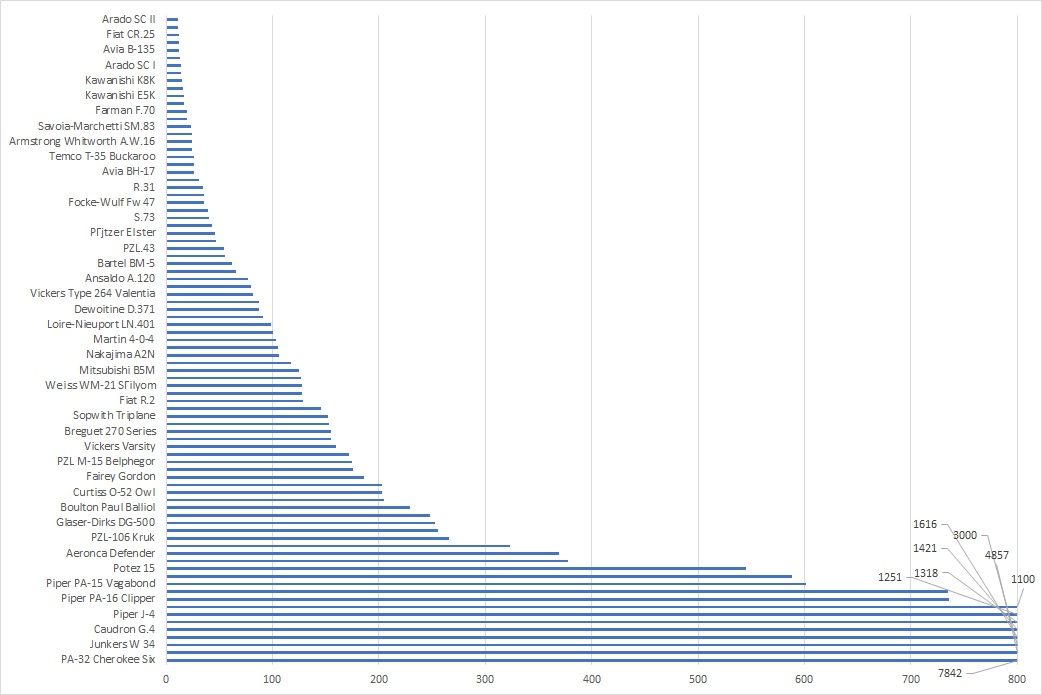
\includegraphics[width=\linewidth]{./chapter/aircraft/Number_of_aircraft_produced_en_2020.jpg}}%

	\caption{Number of aircraft produced by model, 2020.}%
    \label{fig:Number_of_aircraft_produced_en_2020}%
\end{figure*}

Now let's try to answer the question: ``Does \href{https://en.wikipedia.org/wiki/Pareto_principle}{Pareto principle} hold with respect to the 
number of aircraft models"?

In order to build a graph, you must perform the following steps:

\label{question:aircraft_question_2}
\marginnote{
Find the correspondence between the date of foundation and the company.
\\
\begin{tabular}{ l | l }
Company & Foundation date \\ \hline
MiG & 01.01.1939 \\
Vympel & 18.11.1949 \\
Tupolev & 18.12.1939 \\
Sukhoi & 01.01.1922 \\
\end{tabular}
\\
The answer is on page~\pageref{answer:aircraft_answer_2}.
}


\begin{enumerate} 
  \item Calculate the total number of aircraft for all models using the script shown in the listing~\ref{lst:aircraft_listing_5}.

  \index{SPARQL!SUM / Total number of aircraft produced}
  \begin{lstlisting}[ language=SPARQL, breaklines=true,  
                      caption={Total number of aircraft produced\\\hspace{\textwidth}
                          The result contains \num{33 178} aircrafts in 2020.
                          SPARQL query: \href{https://w.wiki/nZi}{w.wiki/nZi}
                          },
                      label=lst:aircraft_listing_5,
                      texcl 
                      ]
  SELECT (SUM(?count) as ?sum) WHERE {
    SELECT ?count WHERE {
      SERVICE wikibase:label {bd:serviceParam wikibase:language "en".}
      ?item wdt:P31 wd:Q11436; # instance of aircraft
        wdt:P1092 ?count. # total aircraft manufactured
    }
  }
  \end{lstlisting}

  \item The X-axis represents the number of aircraft models under consideration (that is, 1 ~--- is the number of manufactured aircraft of the 1st 
  model, 2 ~--- is the sum of aircraft of the 1st and 2nd models, etc.). On the Y-axis, we will plot the percentage of the number of aircraft models 
  produced by all airlines to the total number of aircraft manufactured for all time. Also, along the X axis, we postpone the second scale from 
  0 to 100 \% to make it easier to determine the parameters for the Pareto law.
\end{enumerate}

\begin{figure*}[h]

    \setlength{\fboxsep}{0pt}%
    \setlength{\fboxrule}{1pt}%
    \fcolorbox{gray}{gray}{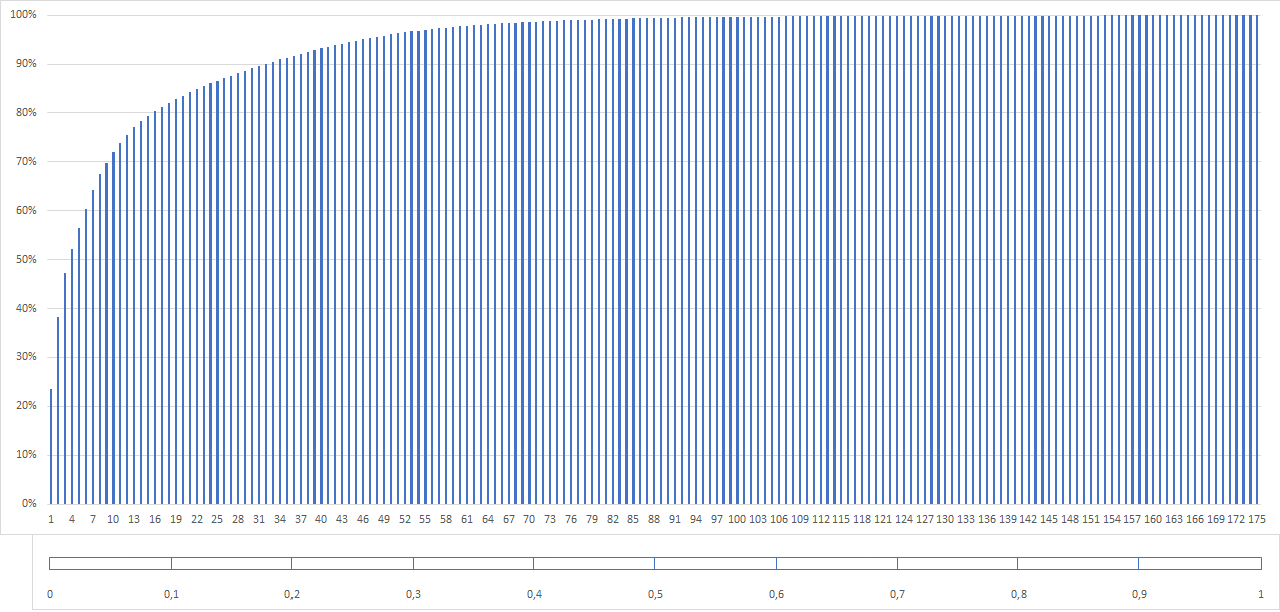
\includegraphics[width=\linewidth]{./chapter/aircraft/Pareto_principle_diargam_en.png}}%

%	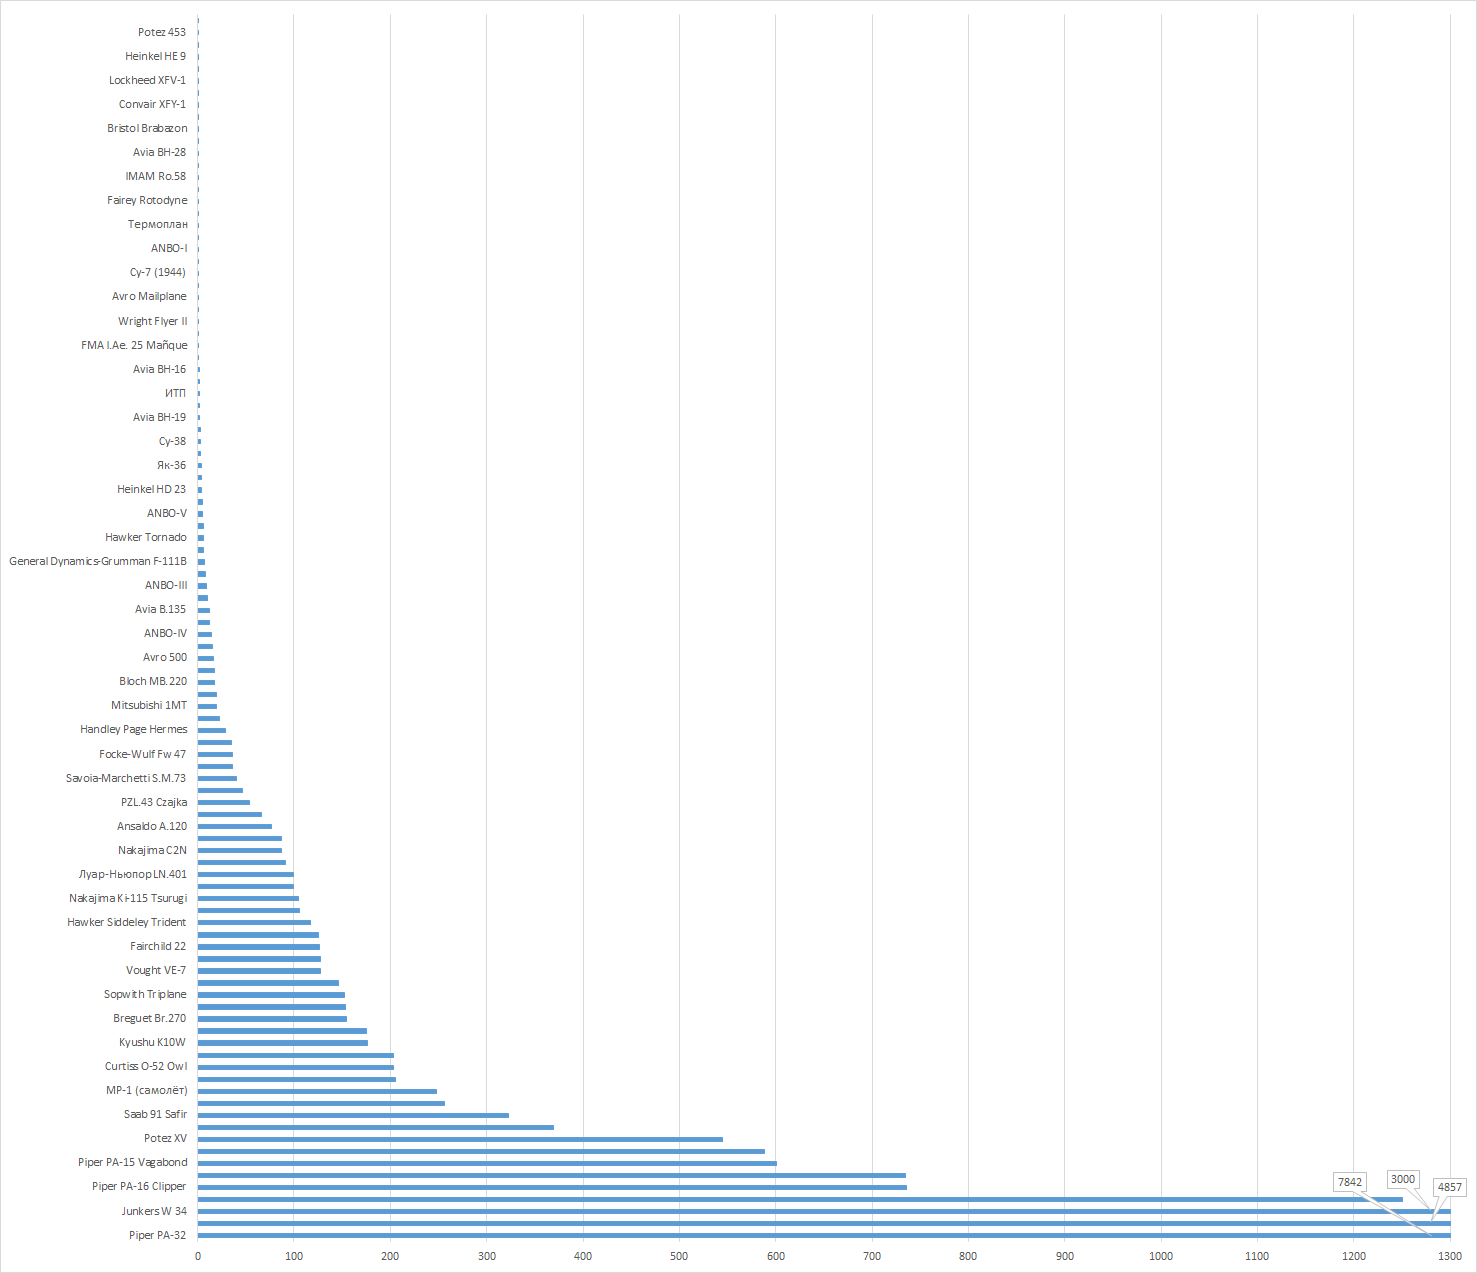
\includegraphics{chapter/aircraft/Number_of_aircraft_produced_ru.png}%
	\caption{Percentage of the number of aircraft models produced by all airlines to the total number of aircraft manufactured for all time, 2020.}%
    \label{fig:Pareto_principle_diargam_en}%
\end{figure*}

According to the graph~\ref{fig:Pareto_principle_diargam_en}, it can be seen that 80\% of all aircraft produced belong to 16 different aircraft 
models, which is 9.2\% of the total number of models. Pareto's law states that: ``20\% of the efforts give 80\% of the result, and the remaining 80\%
 of the efforts - only 20\% of the result." It can be concluded that a stronger law is fulfilled than the Pareto principle regarding the number 
 of aircraft models.

%%%%%%%%%%%%%%%%%%%%%%%%%%%%%%%%%%%%%%%%%%%%%%%%%%%%%%%

\section{Countries of origin of aircraft manufacturers}

Let's build a list of the number of aircraft manufacturers by country. To execute the query~\ref{lst:aircraft_listing_6}, we use the grouping 
by country (GROUP BY) and use the ``Count" function to count the number of productions for each country.

\label{question:aircraft_question_3}
\marginnote{
Find the correspondence between the location of the company's headquarters and the company.
\\
\begin{tabular}{ l | l }
Company & Headquarters \\ \hline
Kazan Helicopters Plant & Kazan \\
Saratov Aviation Plant & Saratov \\
Ulan-Ude Aviation Plant & Ulan-Ude \\
Sukhoi & Moscow \\
\end{tabular}
\\
The answer is on page~\pageref{answer:aircraft_company_headquarters_en}.
}

\index{SPARQL!COUNT / List of the ratio of the number of manufacturers aircraft by country}
\begin{lstlisting}[ language=SPARQL, breaklines=true, 
                    caption={List of the ratio of the \\\hspace{\textwidth} 
						number of manufacturers aircraft by country\\\hspace{\textwidth}
                        The result contains \num{39} records in 2017, 
                        \num{46} records in 2020.\\\hspace{\textwidth}
                        SPARQL query: \href{https://w.wiki/nZu}{w.wiki/nZu}
                        },
                    label=lst:aircraft_listing_6,
                    texcl 
                    ]
# Count manufacture having property country group by country
SELECT ?countryLabel (count(?item) as ?count)
WHERE
{
    ?item wdt:P31 wd:Q936518.   # instance of aerospace manufacture
    ?item wdt:P17 ?country.     # belong to country
    SERVICE wikibase:label {bd:serviceParam wikibase:language "en"}
}
GROUP BY ?country ?countryLabel 
\end{lstlisting}

Having received a list of countries by the number of aircraft manufacturing plants, we can construct a bubble chart 
``The ratio of the number of aircraft manufacturers by country"~\ref{} for clarity. To build it, we execute the request ~\ref{lst:aircraft_listing_7}.

\index{SPARQL!COUNT / Bubble chart ``The ratio of the number of aircraft manufacturers by country"}
\index{Chart!BubbleChart / Bubble chart ``The ratio of the number of aircraft manufacturers by country"}
\begin{lstlisting}[ language=SPARQL, breaklines=true, 
                    caption={Bubble chart\\\hspace{\textwidth}
                        SPARQL query: \href{https://w.wiki/n7E}{w.wiki/n7E}
                        },
                    label=lst:aircraft_listing_7,
                    texcl 
                    ]
#defaultView:BubbleChart
SELECT ?countryLabel (count(?item) as ?count)
WHERE
{
    ?item wdt:P31 wd:Q936518. # instance of aerospace manufacture
  	?item wdt:P17 ?country. # belong to country
    SERVICE wikibase:label {bd:serviceParam wikibase:language "en"}
}
GROUP BY ?country ?countryLabel
\end{lstlisting}

As a result of the query ~\ref{lst:aircraft_listing_7}, a bubble chart will be generated, in which the circles represent countries and their 
sizes correspond to the number of aircraft manufacturers in the specified country. Such a diagram helps to more clearly see the difference 
in the number of aircraft production between countries.

\begin{figure}[h!]
\centering
	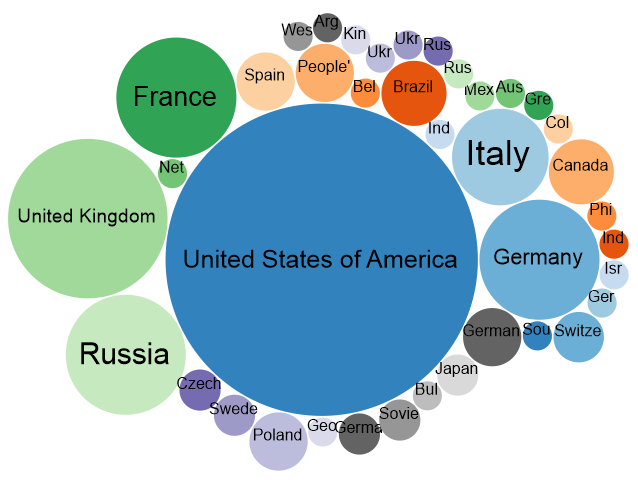
\includegraphics[width=0.7\textwidth]{./chapter/aircraft/Manufacture-with-country_en_2017.png}
	\caption{The ratio of the number of aircraft manufacturers by country, 2017.}
	\label{fig:Manufacture-with-country_en_2017}
\end{figure}

As you can see from the response to the request~\ref{lst:aircraft_listing_7} on (Fig.~\ref{fig:Manufacture-with-country_en_2017}) not all 
aircraft manufacturers are indicated, as evidenced by the data taken from the site \href{https://www.aviationfanatic.com/}{aviationfanatic.com}. 
More information on the lack of data in Wikidata is indicated in the next section of this chapter. Most manufacturers are indicated in the 
USA (115), Great Britain (30), Germany (17), Russia (17) as of May 2017.

\begin{figure}[h!]
\centering
	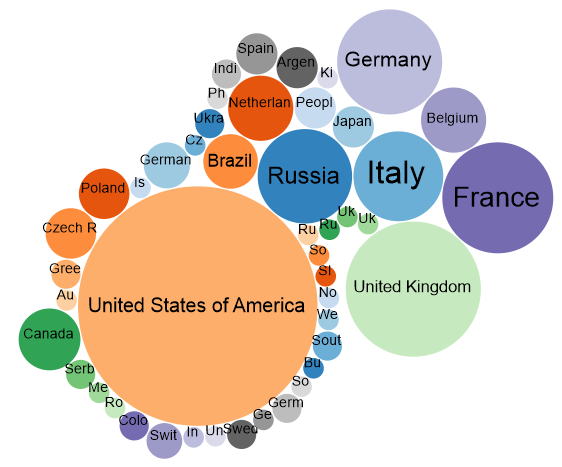
\includegraphics[width=0.7\textwidth]{./chapter/aircraft/Manufacture-with-country_2020_en.png}
	\caption{The ratio of the number of aircraft manufacturers by country, 2020.}
	\label{fig:Manufacture-with-country_2020_en}
\end{figure}

\label{question:aircraft_question_4}
\marginnote{
What is the name of the aircraft, supported in flight by a huge cylinder of flammable, lethal gas, right above the heads of the passengers?
\\
The answer is on page~\pageref{answer:aircraft_question_airship_en}.
}


Comparing two bubble charts for 2017 (Fig.~\ref{fig:Manufacture-with-country_en_2017}) and 2020 (Fig.~\ref{fig:Manufacture-with-country_2020_en}), 
we can conclude that the main aircraft manufacturers are: USA (135 manufacturers) , Great Britain (43), France (29), Germany (26), Russia (21). 
The USA is still the leader, but France in 3 years managed to outstrip Germany, increasing the number of production facilities to 29 
(Germany ~--- 26), thereby taking the 3rd place. But in general, the ratio of aircraft production between different countries remains the same.

%%%%%%%%%%%%%%%%%%%%%%%%%%%%%%%%%%%%%%%%%%%%%%%%%%%%%%%

\section{Completeness of Wikidata}

According to the site \href{https://www.aviationfanatic.com/}{aviationfanatic.com} there are about \num{1700} aircraft manufacturers (2017) 
and \num{1939} (2020), but SPARQL query ~\ref{lst:aircraft_listing_2} returned only 300 records in 2017, and in 2020 ~--- 595 records. 
From this we can conclude that Wikidata is incomplete. Most likely, the manufacturers not listed made too few or none of the aircraft, 
so due to a lack of information they were not included in Wikidata.

Based on the data obtained, you can predict when the data in Wikidata will be complete. In three years, the number of aircraft manufacturers 
increased by 239, representing an annual increase of about 80 aircraft manufacturers. Also during this time, information about 295 aircraft 
manufacturers was entered into Wikidata, that is, about 98 new entries are added annually. Also for 2020, there are no records of \num{1344} 
aircraft manufacturers in Wikidata. Assuming a fixed number of new aircraft manufacturers appear annually and the number of Wikidata entries 
entered annually remains unchanged, we can assume that in about 75 years (i.e. 2095) Wikidata will contain records of all aircraft manufacturers.

The category \href{https://cutt.ly/NhrKnWn}{``Russian Aircraft Companies"} indicates the presence in Russia of 58 aircraft companies in 2017 and 
62 companies in 2020, but at the same time on the website \href{https://www.aviationfanatic.com/}{Aviationfanatic.com} there are 61 
plants in 2017 and 71 in 2020. Among the aircraft building companies in Russia, there are such companies as: \href{https://en.wikipedia.org/wiki/Irkut_Corporation}{Irkut Corporation}, 
\href{https://en.wikipedia.org/wiki/Russian_Aircraft_Corporation_MiG}{Russian Aircraft Corporation MiG}, 
\href{https://en.wikipedia.org/wiki/Tupolev}{Tupolev}.

%%%%%%%%%%%%%%%%%%%%%%%%%%%%%%%%%%%%%%%%%%%%%%%%%%%%%%%

\section{Exercises}

\begin{enumerate}
\item Find the plane with the maximum flight radius.
\item Mark on the political map of the world the location of the main offices of aircraft manufacturers.
\item Find the manufacturer with the most aircraft manufactured using the aircraft manufacturer property \href{https://www.wikidata.org/wiki/Property:P176}{P176}.
\item When was the first aircraft built?
\item Which firms were the first to produce 10, 100 and a thousand aircraft?
\item Draw a chart of the number of aircraft produced by year.
\end{enumerate}
